\subsubsection{Polydiapirism}
\label{sec:benchmark-polydiapirism}

\textit{This section was contributed by Cedric Thieulot.}

Diapirs are a type of geologic intrusion in which a more mobile and ductily deformable material (e.g., salt)
is emplaced into (brittle) overlying rocks. As salt domes are capable of trapping petroleum and
natural gas these structures have been extensively studied \cite{jahu17}.

We consider in this experiment the three-layer viscous Rayleigh-Taylor instability proposed
by Weinberg and Schmeling \cite{wesc92}
and we focus in what follows on the case II of that publication.
The domain is a 2D Cartesian box of size $2.24~\si{m} \times 1~\si{m}$.
Gravity is Earth-like ($9.81~\si{\meter\per\square\second}$).
Boundary conditions are free-slip on the sides and top and no-slip at the bottom.
All three layers are initially horizontal. The top layer (fluid 1) has a thickness of
$0.75~\si{m}$, a viscosity $\eta_1=100~\si{\pascal\second}$ and a density $\rho_1=100~\si{\kg\per\cubic\meter}$.
The middle layer (fluid 2) has a thickness $0.125~\si{\meter}$ with $\rho_2=90~\si{\kg\per\cubic\meter}$ and $\eta_2=1~\si{\pascal\second}$.
The bottom layer (fluid 3) has a thickness $0.125~\si{\meter}$ with $\rho_3=89~\si{\kg\per\cubic\meter}$ and $\eta_3=1~\si{\pascal\second}$.
The two interfaces between the layers are perturbed by a random noise of amplitude $\pm 0.001~\si{m}$.
Since fluid 3 is lighter than fluid 2 and fluid 2 is lighter than fluid 1, both interfaces are unstable.
We observe that interface 2-3 deforms first, produces domes which are subsequently incorporated in the domes
being generated at the interface 1-2, as shown in Figure~\ref{fig:polydiapirs_density}.
The root mean square velocity (Figure~\ref{fig:polydiapirs_vrms}) shows two slopes in the early stages ($t<50~\si{\second}$)
corresponding to the two different growth rates of the interfaces, as explained by linear stability analysis \cite{wesc92,ramb81}.

\begin{figure}
    \centering
    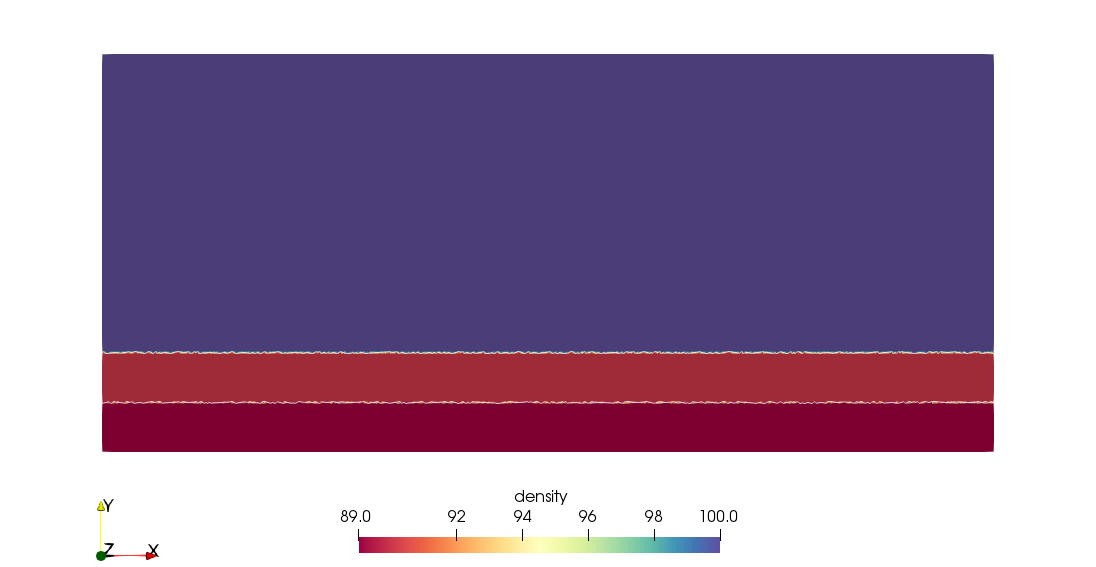
\includegraphics[width=0.48\textwidth]{cookbooks/benchmarks/polydiapirs/doc/diapirs0000.png}
    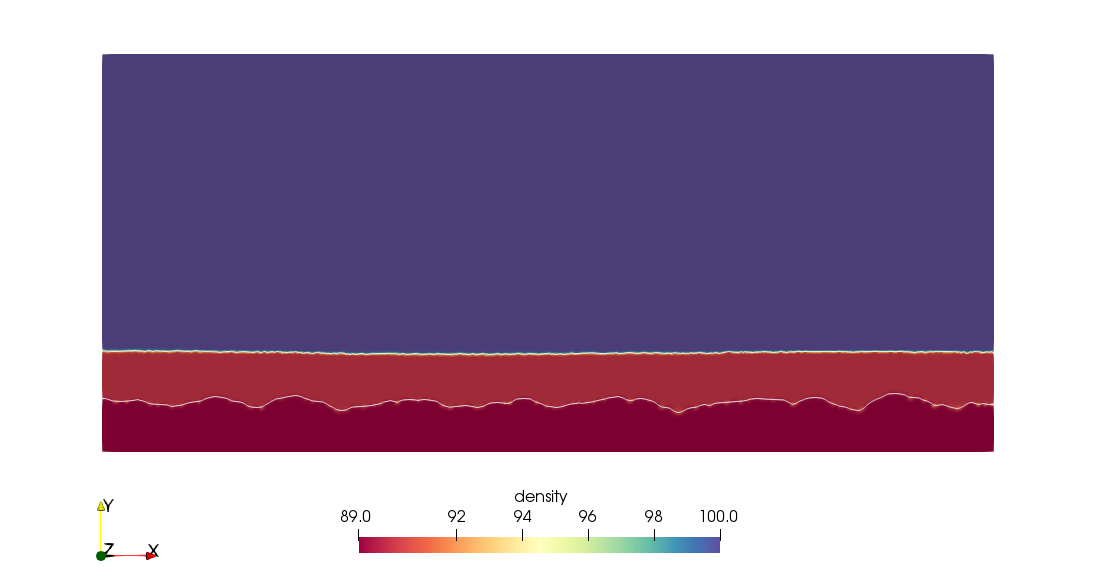
\includegraphics[width=0.48\textwidth]{cookbooks/benchmarks/polydiapirs/doc/diapirs0005.png}
    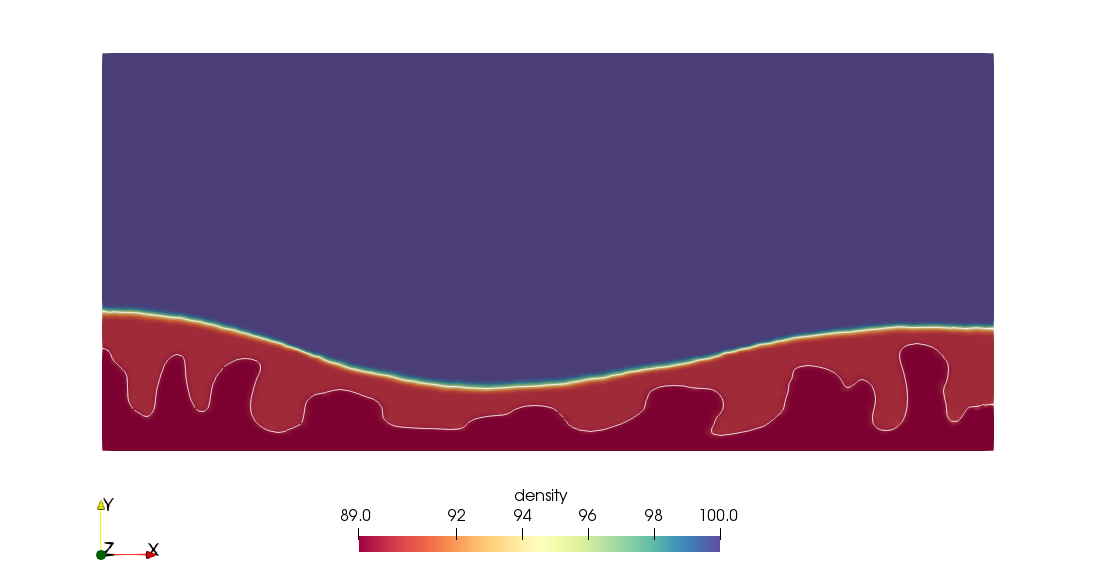
\includegraphics[width=0.48\textwidth]{cookbooks/benchmarks/polydiapirs/doc/diapirs0010.png}
    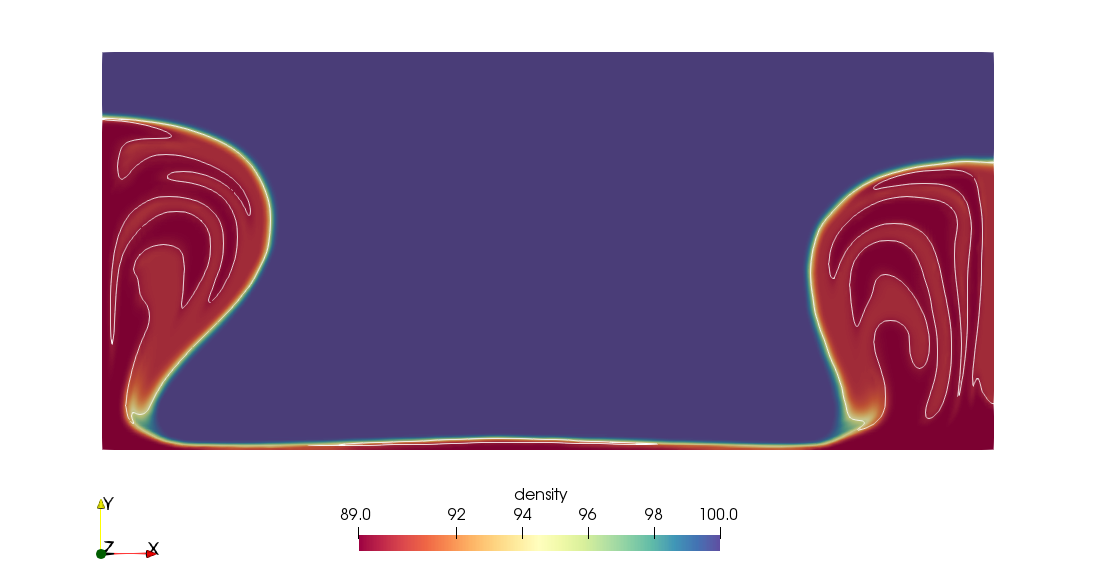
\includegraphics[width=0.48\textwidth]{cookbooks/benchmarks/polydiapirs/doc/diapirs0015.png}
    \caption{\it Polydiapirism benchmark: Density field at $t=0,25,50,75~\si{\second}$.}
    \label{fig:polydiapirs_density}
\end{figure}

\begin{figure}
    \centering
    \includesvg[width=0.75\textwidth]{cookbooks/benchmarks/polydiapirs/doc/vrms.svg}
    \caption{\it Polydiapirism benchmark: Root mean square velocity as a function of time}
    \label{fig:polydiapirs_vrms}
\end{figure}


